The focus of this chapter is on the problem of \textbf{deriving a mathematical model} of $N$ identical LTI agents $S_i$, $i=1,...,N$. The agents can be described:
\begin{itemize}
    \itemsep0em
    \item In the \textbf{Discrete Time Domain} ($t\in\mathbb{R}^+$):
    \begin{align*}
        &\text{state-space description} &\quad
        &\begin{cases}
            \dot{x}_i(t)=Ax_i(t)+Bu_i(t)\\
            y_i(t)=Cx_i(t)
        \end{cases}\\
        &\text{transfer function description} &\quad
        &H(s)=C(sI-A)^{-1}B
    \end{align*}
    \item In the \textbf{Continuous Time Domain} ($k\in\mathbb{N}$):
    \begin{align*}
        &\text{state-space description} &\quad
        &\begin{cases}
            \dot{x}_i(k)=Ax_i(k)+Bu_i(k)\\
            y_i(k)=Cx_i(k)
        \end{cases}\\
        &\text{transfer function description} &\quad
        &H(z)=C(zI-A)^{-1}B
    \end{align*} 
\end{itemize}

\section{What kind of model?}
\noindent
Different approaches are available which are based on \textbf{physical insights} and/or \textbf{input-output collected experimental data}. We can split this approaches mainly into three groups:
\begin{enumerate}
    \item \textbf{First-principle modeling}: here the structure for the system is derived only by applying the physics, moreover the equation structure is known and taken from the physic theory and, sometimes \textbf{the value of the parameter are known}, other times dedicated experiments are conducted in order to retrieve them with a certain approximation; such models are also knows as \textbf{white-box models}.
    \item \textbf{System identification}: is an approach that we find on the opposite part. In fact, here the model is derived by using \underline{\textbf{both}} input-output \textbf{collected data} and some \textbf{a-priori information} which are fundamental. The parameters come up as an \textbf{output} of the SysID procedure but do not have a physical meaning, such models bring to \textbf{black-box models}. 
    \item \textbf{Mixed approach}: here the structure of the equation is taken from the Physics (even if partially), the physical parameter to be estimated are meaningful and come up, again, as output of the procedure. The techniques which are based on these considerations are  \textbf{gray-box models}.
\end{enumerate}

\section{System Identification: black-box general setting}
\noindent
In general, the first approach which use \textbf{first-principle modeling} is not so used because the equation of the Physics are always \textit{approximation of the reality}, sometimes peculiar aspects - not trivial to mathematically formulate - can be wrongly neglected leading to bad models.\\
The \textbf{gray-box approach} is rarely used because similarly than the first case impose strong and not mild constraints on the structure of the equations and on the parameter which being related to the physical meaning cannot be arbitrarily chosen. (We will go more in details on such aspect later).\\
The most general approach is represented by the \textbf{System Identification approach} in which:
\begin{enumerate}
    \item Input-Output data are exploited, these are affected by \textit{measurement noise};
    \item Some a-priori assumption are used; 
    \item The \textbf{most natural} description, since input and output data are employed, is the \textbf{transfer function}. Finally, using the \textit{realization theory} we can obtain the state state description.
\end{enumerate}

\hspace*{-5mm}
\begin{tikzpicture}
\node [mybox] (box){%
    \begin{minipage}{.96\textwidth}     %Larghezza del box
        {\Large{
            \begin{equation*}
                \begin{aligned}
                \textsf{\textbf{State-Space}}
                &\overset{\mathcal{L}}{\Longrightarrow}
                \textsf{\textbf{Transfer function }}\\
                \textsf{\textbf{Transfer function }}
                &\overset{\text{\tiny{Realization}}}{\Longrightarrow}
                \textsf{\textbf{State-Space }}
                \end{aligned}
            \end{equation*}
        }}
    \end{minipage}
};
\end{tikzpicture}%

\vspace{0.2cm}
\noindent
This approach is very used because of a \textbf{great flexibility}, for instance we need only some weak assumption based on physical insights.
Now, since the input-output data are \textbf{samples} of some signals we can start to discuss the System Identification(SysID) procedure for \textit{discrete-time systems}.\\
Without loss of generality we can say that the system to be identified (which may be in general nonlinear) can be described by using the \textit{regression form}
{\large{
    \begin{equation} \label{eq: regression_form}
        \begin{aligned}
            y(k)=&f(y(k-1), y(k-2), ...,y(k-n), \\
            &u(k), u(k-1), ..., u(k-m)), \ m\le n
        \end{aligned}
    \end{equation}
}}

Where $n$ is the order of the system, while $m$ is frequently assumed to be equal to $n$. In some situation I know the value of $n$, in other situation One can choose a value for $n$ which is \textbf{sufficiently large}, then the data will guide us on the choice of the \textbf{system order}. $u(k)$ and $y(k)$ are the error-free signals.\\
A quite general setting for the SysID procedure can be surely the \textbf{Error-in-Variable (EIV)} one in which the measurement noise affects both the input and output \textbf{collected data}. 

\begin{figure}[h]
    \centering
    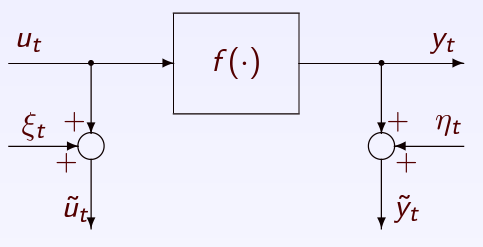
\includegraphics[scale=0.77]{images/EIV.png}
    \caption{EIV System Identification setup}
\end{figure}

\vspace{0.5cm}
%description of the terms in the figure
\noindent
How we outline before:
\begin{itemize}
    \itemsep0em
    \item[$\square$] The function $f(\cdot)$ is that to be identified;
   \item[$\square$] The terms $\tilde{u}_t$ and $\tilde{y}_t$ are the input-output collected data, which are both the real quantities ($u_t$ and $y_t$) to which is added 
   \item[$\square$] The \textbf{noise term} indicated with $\xi_t$ and $\eta_t$.
\end{itemize}

\noindent
At this point, in order to be more specific, let us clarify some aspects about the important \textbf{a-priori assumptions} which are basically of three types:
\begin{enumerate}
    \itemsep0em
    \item On which part of the system the noise enters?
    \item Assumption on the class $\mathcal{F}$ of the function $f(\cdot)$ to identify; 
    \item Is the noise of a certain type? (hypotesis on statistichal distribution, boundness, energy...)
\end{enumerate}



\subsection{Example (noise free): 2$\mathbf{^{\text{nd}}}$ order LTI system}
We have said that the most natural way to express the structure of $f(\cdot)$ is by using a \textbf{transfer function}.  But, \textbf{How can we obtain it from the regression form?} We can show it using an example.\\
Let us consider that on the system to be identified we have the following \underline{a-priori assumptions}:
\begin{enumerate}
    \item There is no noise, so $\tilde{u}_t=u_t$ and $\tilde{y}_t=y_t$;
    \item The system is \textit{linear}, in this way we have choose the class $\mathcal{F}$ for the function $f$
    \item The order of the system is $n=2$ and $m=n$.
\end{enumerate}
Using the assumption (3), the equation (\ref{eq: regression_form}), in this case becomes
\begin{equation}
    y(k) = f(y(k-1)+y(k-2)+u(k)+u(k-1)+u(k-2))
\end{equation}
Moreover, from the moment we know that the function is linear, we can express it in the following way:
\begin{equation} \label{eq: reg_linear}
    y(k)=-\theta_1y(k-1)-\theta_2y(k-2)+
    \theta_3u(k)+\theta_4u(k-1)+\theta_5u(k-2)
\end{equation}
Using the \textbf{backward shift operator} according to which $s(k-r)=q^{-r}s(k)$, we rewrite it as
\begin{align*}
    &y(k)=-\theta_1 q^{-1} y(k) -\theta_2 q^{-2} y(k) 
    + \theta_3u(k) + \theta_4 q^{-1} u(k) + \theta_5 q^{-2} u(k) \iff \\
    &y(k) +\theta_1 q^{-1} y(k) +\theta_2 q^{-2} y(k) = \theta_3u(k) + \theta_4 q^{-1} u(k) + \theta_5 q^{-2} u(k)
    \iff\\
    &y(k) [1+\theta_1 q^{-1}+\theta_2 q^{-2}] = u(k) [\theta_3+\theta_4q^{-1}+\theta_5q^{-2}] \iff\\
    & y(k) = \frac{\theta_3+\theta_4q^{-1}+\theta_5q^{-2}}{1+\theta_1 q^{-1}+\theta_2 q^{-2}} u(k)
\end{align*}
\noindent
There is a (not trivial) formal proof that the backward shift operator is equivalent to the delay $z^{-1}$ in the $\mathcal{Z}$-transform domain. It is immediate now, to find the transfer function 
\begin{equation}
    G(z) = \frac{
        \theta_3 z^2 + \theta_4z + \theta_5
    }{
        z^{2}+\theta_1z + \theta_2
    }
\end{equation}
Then, we have understood that passing through the \textit{regression form} we can obtain a \textbf{transfer function} using the a-priori assumptions and the I/O collected data.

\subsection{Estimation of the parameters}
Assuming, for the moment, we can experimentally collect I/O data without adding any noise, how can we obtain the parameters $\theta_1, ..., \theta_5$? The equation (\ref{eq: reg_linear}) have 5 unknowns, we may find a unique solution by adding other equations. \\
Before start, we have to collect a sufficient number of samples in order to compute $y(k)$, here we need the measurement $y(1), y(2), u(1), u(2)$ in order to compute $y(3)$.[In general if $n$ is the order of the system we start computing $y(k)$ from the instant $k=n+1$]. It is obtained:
\begin{align*}
    &y(3)=-\theta_1y(2)-\theta_2y(1)+\theta_3u(3)+\theta_4u(2)+\theta_5u(1)\\
    &y(4)=-\theta_1y(3)-\theta_2y(2)+\theta_3u(4)+\theta_4u(3)+\theta_5u(2)\\
    &\vdots\\
    &y(7) = -\theta_1y(6)-\theta_2y(5)+\theta_3u(7)+
    \theta_4u(6)+\theta_5u(5)
\end{align*}
that it can be rewritten in matrix form as
\begin{equation} \label{eq:sys_eq}
    \underbrace{\begin{bmatrix}
        y(3)\\y(4)\\\vdots\\y(H)
    \end{bmatrix}}_{y} 
    =\underbrace{ 
    \begin{bmatrix}
        y(2)&y(1)&u(3)&u(2)&u(1)\\
        y(3)&y(2)&u(4)&u(3)&u(2)\\
        &\vdots&\vdots&\vdots&\vdots\\
        y(H-1)&y(H-2)&u(H)&u(H-1)&u(H-2)
    \end{bmatrix}}_{A} \underbrace{\begin{bmatrix}
        \theta_1\\\theta_2\\\vdots\\\theta_H
    \end{bmatrix}}_{\theta}
\end{equation}
[In our case$H=7$]. If the matrix $A$ is invertible we can find the solution $\theta$ only by inverting the system
\begin{equation} \label{eq: inversion}
    \theta = A^{-1}y
\end{equation}
In order to guarantee that $A$ is invertible one might think that we can apply a \textit{random} input sequence, so that the columns of the matrix would be linearly independent, but it is not realistic because we want to excite the system with a particular class of signals, moreover \textbf{it is not necessary} doing such assumption: it is known what is for example the \textbf{step response} of a second-order LTI systems. There is a transient in which the output of the system oscillates a lot: 
\begin{quote}
    it is practically impossible to obtain a matrix whose columns are linearly dependent, even if the system is excited with a very simple signal of the type $u(k)=c\in\mathbb{R}$ the response has oscillations which ensure us, at a certain extent, to take independent measurements. Clearly, \textbf{the more exciting the input, the more information can be retrieved by analysing the output}.
\end{quote}

\subsection{Black-box models vs Gray-box models}
We have analysed a bit the main features of the SysID approach, so that some more specific comparison can be done with the gray-box approach.\\
The a-priori assumption on the \textit{linearity} of the system allowed us to pick a function in which \textbf{the parameters appear linearly in the model}, on the other hand their meaning is not relevant.\\
If we used more the physical insights, we are constraining the structure of the equations and so of the transfer function. For example, from the Physics one can  find that
\begin{equation*}
    G(s)=\frac{
        \sqrt{\gamma_1}s^2+\gamma_2s+\gamma_3/\gamma_4
    }{
        s^2+\frac{1}{\gamma_3}s+\gamma_5^2
    }
\end{equation*} 
Here we find that:
\begin{itemize}
    \item The \textbf{system} associated with $G(s)$ is \textbf{linear}; 
    \item The \textbf{parameters} appear in the equation \textbf{non-linearly}, and here they are meaningful because are the parameters derived from the Physics.
\end{itemize}
In general, it  is not trivial to find the solution in the case that \textbf{the system is not linear-in-parameters}, so it clearly appears that a SysID approach, without loss of generality, could bring to a simpler solution. What we lose is the meaning of the estimated parameters.

\subsection{The role of the a-priori information}
Introducing the System Identification approach, we have remarked that is crucial that \textit{collected data} and \textit{a-priori assumption} are used in order to estimate the parameters. \textbf{What if we do not use the physical insights to retrieve the structure of the system?} Let us give an example for a \textbf{static} and \textbf{non-linear} system.
\begin{equation*}
    y(k)=\theta_1u(k) + \theta_2 u(k)^2 + \theta_3 u(k)^3 + \theta_4 u(k)^4 + \theta_5 u(k)^5
\end{equation*}
Even if the equation linked to the system is \textbf{non-linear}, the parameters appear \textbf{linearly} in the equation so that we can apply the same approach of the first example, we have five parameters and we need 5 equation, furthermore, since the system is static we need only 5 samples for $u$ and 5 samples for $y$:
\begin{align*}
    &y(1)=\theta_1 u(1)+ \dots + \theta_5 u(1)^5\\
    &y(2)=\theta_2 u(2)+ \dots + \theta_5 u(2)^5\\
    &\vdots \quad = \quad \quad \vdots \\
    &y(5)=\theta_2 u(5) + \dots + \theta_5 u(5)^5
\end{align*}
\noindent
That in matrix form
\begin{equation*}
    \begin{bmatrix}
        y(1)\\y(2)\\\vdots\\y(5)
    \end{bmatrix}=\begin{bmatrix}
        u(1)&u(1)^2&...&u(1)^5\\
        u(2)&u(2)^2&...&u(2)^5\\
        \vdots&\vdots&\vdots&\vdots\\
        u(5)&u(5)^2&...&u(5)^5
    \end{bmatrix} \begin{bmatrix}
        \theta_1\\\theta_2\\\vdots\\\theta_5
    \end{bmatrix}
\end{equation*}
If we invert the system by applying the equation (\ref{eq: inversion}) we will obtain the parameter $\theta$, BUT \textbf{what if we use the resulting $y(k)$ to predict the behaviour of the system?} We neglected the relevant fact the system is of the second order! At this point:
\begin{enumerate}
    \item If we use the collected data to do the prediction, it will be correct for sure \textbf{(we built the model relying only on them)}
    \item If we apply a certain sequence $u(k)$ to the system $\mathcal{S}$ and we take the corrensponding $y(k)$ samples, we will note that the prediction done according to the identified model is \textbf{completely wrong!}.
\end{enumerate}
Conclusion:
\begin{quote}
    \large{\color{blue}
        In the System Identification procedure if we rely only on the input-output collected data, we will \textbf{overfit} the data, this is the reason why \textbf{the a-priori assumptions act a fundamental role in the identification procedure}.
    }
\end{quote}


\subsection{From the ideal situation to the real experiment}
Only in order to simplify the explanation, we started with the assumption that the input-output collected data were \textbf{noise-free}. In the real-world experiments we cannot do this assumption! Always we have that the collected data is:
\begin{align}
    &\tilde{u}_t = u_t+\xi_t\\
    &\tilde{y}_t = y_t+\eta_t
\end{align}
Making us guided from an example, this situation will be more clear. Let us consider a very simple  example: a \textbf{resistor} through which a current $i(t)$ is passing. The input $u(t)$ is the current $i(t)$ itself, while the output is clearly the voltage $v(t)$ on the resistor. The simple equation which describe this system is 
\begin{equation}
    y(k) = \theta u(k)
\end{equation}
Following the procedure we did before and considering that only the output $\tilde{y}(k)$ is affected by the noise, we have a \textbf{single parameter}; then a single equation, and a \textbf{single sample} to be taken of the input and the output, might be sufficient in order to obtain an \textbf{estimate} $\hat{\theta}$ of the parameter, which in this case we know that is a \textbf{resistance}.
If we had used the real $u(k)$ and $y(k)$, the $\theta$ parameter would have been
\begin{equation}
    \theta = \frac{y(k)}{u(k)}
\end{equation}
but, if we apply our naive approach using the collected data which are corrupted by the \textbf{measurement noise} we obtain
\begin{equation}
    \hat{\theta} = \frac{\tilde{y}(k)}{u(k)} = 
    \frac{y(k)}{u(k)}+\frac{\eta{k}}{u(k)} = \theta + \frac{\eta(k)}{u(k)} \ne \theta
\end{equation}
Conclusion:
\begin{quotation}
    If we use a single sample, we will obtain for sure a wrong estimate of the single parameter $\theta$ $\to$ a \textbf{wrong model}. We need more samples and we will look for a $\theta$ which is providing the \textbf{best-fitting} of the data.
\end{quotation}

\noindent
In order to exit from this \textbf{wrong situation}, we have to collect for sure more \textit{input-output} pairs in a number $H \gg 2n+1$, where $2n+1$ given a system of order $n$ is the number of parameters to estimate $\to$ the output of our system identification procedure. However at this point we cannot apply anymore the equation (\ref{eq: inversion}) because the matrix $A$ becomes a tall matrix, which cannot be inverted! We use the Moore-Penrose pseudo inverse defined as
\begin{equation*}
    A^\dagger = (A^TA)^{-1}A^T
\end{equation*}
and we can solve the problem by simply substituting the inverse with the pseudoinverse:
\begin{equation} \label{eq: LS_solution}
    \hat{\theta} = A^\dagger y = (A^TA)^{-1}A^T y
\end{equation}
This is the solution of the Least-Squares problem (LS) to the equation (\ref{eq:sys_eq})
\begin{equation}
    \hat{\theta} = \text{arg}\min_\theta \Vert A\theta-y\Vert_2^2
\end{equation}
In this way $\hat{\theta}$, in the context of System Identification, is the LS estimate of the \textit{parameter vector}.\\
This formulation of the problem has interesting properties if some hypothesis are satisfied:
\begin{enumerate}
    \item The error apper in the equation as an additive term $e(k)$ called the \textbf{equation error}; 
    \item The $e(k) k=1,...,H$ represents a white gaussian noise, that is the samples are \textit{indipendent and identically distributed} (iid).
\end{enumerate}
If such assumption are fullfilled, then
{\large{
    \begin{equation}
        \lim_{H\to\infty} \mathbb{E}\big[\hat{\theta}\big] = \theta
    \end{equation}
}}
Where $\theta$ is the \textbf{true parameter vector}. The Least Square approach, no matter what are the dimension of the matrix is \textbf{very fast}, moreover there is also an \textit{online recursive way} to compute them.\\
At this point we are assuming that:
\begin{align*}
    &y(k)=-\theta_1y(k-1)-\theta_2y(k-2)-...-\theta_ny(k-n)+\theta_{n+1}u(k)+...+\theta_{n+m+1}u(k-m) + e(k) \iff \\
    &y(k)=-\theta_1 q^{-1}y(k)-\theta_2 q^{-2}y(k)-...-\theta_n q^{-n}y(k) + \theta_{n+1}u(k) + ... + \theta_{n+m+1} q^{-(n+m+1)} u(k) + e(k) \iff \\
    &y(k) \big(1+\theta_1 q^{-1}+...+\theta_n q^{-n} \big) = u(k) \big( \theta_{n+1} q^{n+1}+...+\theta_{n+m+1}  q^{n+m+1} \big) + e(k) \iff \\
    &y(k) D_d(q^{-1})=u(k)\ N_d(q^{-1}) + e(k) \iff 
    y(k)=\frac{N_d(q^{-1})}{D_d({q^{-1}})} u(k) + \frac{1}{D_d(q^{-1})}e(k) \quad _\blacksquare
\end{align*}
This last step we did tells us that the output of the system \textbf{to be identified} depends:
\begin{enumerate}
    \item On the transfer function to be identified $\frac{N_d(q^{-1})}{D_d({q^{-1}})}$ (this is ok);
    \item On the error filtered by the transfer function $\frac{1}{D_d(q^{-1})}$ which depends directly on something to be identified  yet!
\end{enumerate}

\noindent
\textbf{Conclusion}
The Least-Squares estimator used to solve the SysID problem has some advantages: fast convergence and simplicity, however in order to be used requires \textbf{strong assumption} on the error, moreover even if this can be obtained, having an acceptable estimate requires the collection of a big quantity of data. 
\begin{center}
    \color{red}
    We need an approach where:
    \begin{enumerate}
        \item A \textbf{small amount of data} is required; 
        \item \textbf{mild assumption} on the error has to be done.
    \end{enumerate}
    These needs leads to the \textbf{Set-Membership System Identification} theory.
\end{center}


  






